It is of primary interest to apply the \gls{qmla} algorithm to real-life, experimental systems. 
In this chapter we devise an \gls{es} to operate in conjunction with experimental data 
    in order to characterise an electron spin in an \gls{nv} centre in diamond.
In particular, we model, through Hamiltonian terms, interactions between the spin and 
    the spin bath in which it resides,
    so that \gls{qmla} is finding an effective model for the open system dynamics.
\par

Here we will first introduce a basic picture of \glspl{nvc}, 
    using basic but nonstandard nomenclature for simplicity;
    for thorough descriptions of the underlying physics, readers are referred to \cite{doherty2013nitrogen}.
We next discuss the target system with respect to its modelling, 
    determining the suitable terms which \emph{might} represent the \gls{nvc}'s interactions, 
    to inform the starting point for the \gls{qmla}.
Finally we describe the implementation of an \gls{es} for the examination of the \gls{nvc},
    and the results of the \gls{qmla} procedure. 

\section{\Glsentrylong{nvc}}
\label{sec:nv_centres}

\gls{nv} centers are point defects in diamond, 
    occuring naturally \cite{davies1976optical} or synthetically \cite{meijer2005generation, edmonds2012production}.
A substitutional \gls{nitrogen} isotope is embedded in a lattice of carbon atoms in diamond, 
    adjacent to a lattice vacancy, 
    such that it is surrounded by three \glspl{carbon} \cite{lenef1996electronic}. 
Of the \gls{nitrogen} atom's five valence electrons, three bond with nearby \glspl{carbon};
    the remaining two unbonded electrons for a lone pair and can be thought of as a single spin-$\frac{1}{2}$ particle. 
The adjacent lattice vacancy has three unbonded electrons, 
    two of which bond together leaving a single unpaired electron.
The single electron in the lattice vacancy, together with the effective lone pair of the \gls{nitrogen}, 
    form a a system of two spin-$\frac{1}{2}$ particles.
Such systems have been thoroughly studied; 
    of particular interest are the resultant \emph{triplet} states, 
    i.e. the allowed permutations of the two particles with total quantum spin $S=1$, 
    with magnetic spin multiplicity allowing $m_s = {-1, 0, 1}$, 
    giving rise to three distinct energy levels for the system. 
\par 

A \emph{manifold} is a set of states differing only slightly, 
    for example states near the absolute ground state manifold might differ only in magnetic spin quantum number,
    and can be characterised as the ground state manifold. 
We consider two principle manifolds of the system:
    the ground state and excited manifolds, each consisting of 
    three states, corresponding to the allowed values for magnetic spin $m_s$, see \cref{fig:nv_centre_energy_levels}a. 
For brevity, we denote states with reference to their magnetic spin and manifold, 
    e.g. the state in the ground state manifold with $m_s=0$ is denoted $\ket{m_s=0}_g$. 
In the absence of a magnetic field, the states corresponding to $\ket{m_s=\pm1}$ are degenerate, 
    but in the presence of a magnetic field, $B$, they have distinct energy levels, 
    referred to as the Zeeman effect, \cref{fig:nv_centre_energy_levels}b. 
\par 

We designate the state $\ket{m_s=0}_g$ as the basis state $\ket{0}=\icol{1 \\ 0}$, 
    and $\ket{m_s=-1}_g$ as $\ket{1}=\icol{0 \\ 1}$, 
    such that we have defined a qubit and computational basis, \cref{fig:nv_centre_energy_levels}d.
By shining a laser of $532$nm (green) on the \gls{nvc}, it is excited to the excited manifold, 
    from which it decays back to the ground state manifold. 
Importantly, the process of this decay can be exploited for the preparation of the \gls{nvc} in 
    the computational basis state $\ket{0}$. 
That is, the dominant decay process from $\ket{m_s=0}_e$ is 
    spin-preserving, so it ends in $\ket{m_s=0}_g$. 
On the other hand, had the \gls{nvc} been in the $\ket{m_s=\pm1}_e$,
    the dominant decay process is through a shelving (singlet) state, 
    and does not preserve spin, such that it also decays to the $\ket{m_s=0}_g$.
Therefore, irrespective of the initial state, 
    by shining the green laser on the \gls{nvc}, 
    it is most likely that it has been prepared in $\ket{m_s=0}_g = \ket{0}$, 
    providing us a starting point from which to perform computation.
\par 

The difference in energy between $\ket{0}$ and $\ket{1}$ is addressible optically: 
    by shining a \gls{mw} pulse at the \gls{nvc}, we can oscillate the qubit between the two levels. 
Likewise, having initialised the state to $\ket{0}$, we can perform a $\nicefrac{\pi}{2}$ rotation 
    about the logical $z$-axis, by running the \gls{mw} laser for half the time, 
    resulting in the state $\ket{+}$. 
We can similarly devise \gls{mw} radiation to achieve quantum gates and operations on our \gls{nvc} qubit.
We depict these cycles in \cref{fig:nv_centre_energy_levels}c. 
\par

\begin{figure}
    \begin{center}
        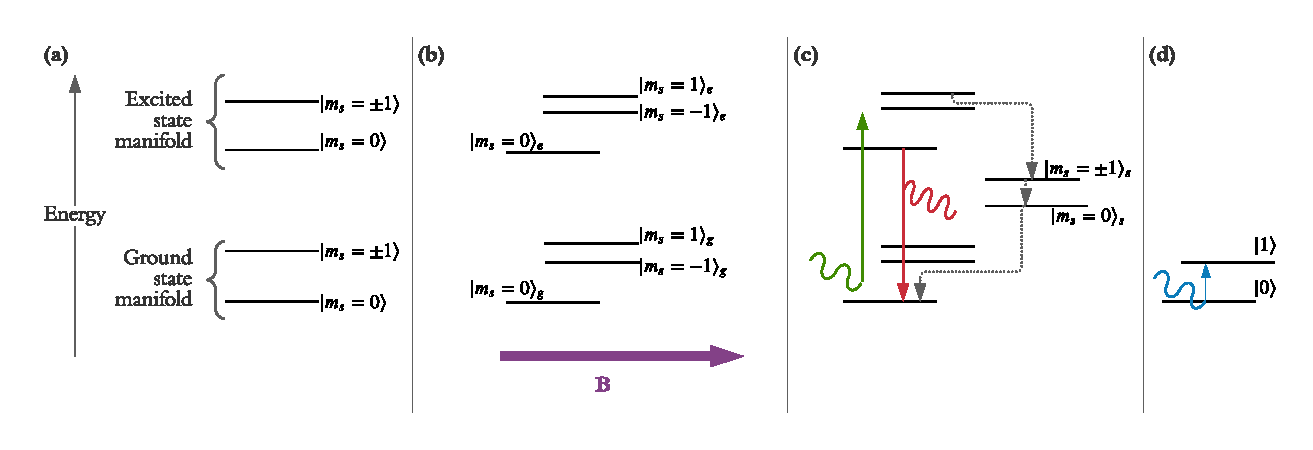
\includegraphics[width=0.75\linewidth]{experimental_study/figures/nv_centre_cartoon.pdf}
    \end{center}
    \caption[\Glsentrylong{nvc} energy levels.]{
        Simplified depiction of energy levels of the \glsentrylong{nvc}, corresponding to its triplet state. 
        \textbf{a}, With no external field, the system simply has excited and ground-state manifolds, 
        each of which consist of two energy levels depending on the magnetic spin, $m_s$.
        \textbf{b}, In the presence of a magnetic field (purple, $B$), the magnetic spins have distinct energy levels, 
        i.e. Zeeman splitting. 
        States are denoted by their magnetic spin and subscripted by their manifold. 
        \textbf{c},  Application of a green ($532nm$) laser excites the \gls{nvc} from any of the states in the 
        ground state manifold to the excited manifold. 
        The dominant decay mechanism for the excited states are shown: 
            (i) $\ket{m_s=0}_e \rightarrow \ket{m_s=0}_g$ (red line) through the emission of a red ($637nm$) photon;
            (ii) $\ket{m_s=\pm 1}_e \rightarrow \ket{m_s=0}_g$ (dotted grey lines) via the shelving manifold which allows for non-spin-preserving transition, 
            and does not emit a photon. 
        \textbf{d}, Computational basis states $\ket{0}$ and $\ket{1}$ are assigned to the two lowest energy states.
            The difference in energy between these states is such that a microwave (MW, blue) photon
            can trigger transition from $\ket{0}$ to $\ket{1}$, as well as states in between such as $\ket{+}$, 
            allowing for the implementation of quantum logic gates. 
    }
    \label{fig:nv_centre_energy_levels}
\end{figure}


We can further exploit the decay mechanism to compose a readout procedure, 
    to infer the population of $\{\ket{0}, \ket{1}\}$ at a given instant, 
    for example following the application of gates to the system. 
We know that the excitation due to the green laser is spin-preserving, 
    i.e. when the \gls{nvc} has been excited to $\ket{m_s=0}_e$, 
    it had originated in $\ket{m_s=0}_g$.
We also know that the decay $\ket{m_s=0}_e \rightarrow \ket{m_s=0}_g$ is spin preserving, with the emission of 
    a red photon: by simply counting the number of photons emitted, we quantify the population of $\ket{0}$
    at the time of query. 
On the contrary, when the $\ket{m_s=-1}_g$ is excited, spin is also preserved, 
    so it goes to $\ket{m_s=-1}_e$;
    but $\ket{m_s=-1}_e$ decays 
    through the shelving state as outlined earlier, 
    \emph{without} the emission of a photon. 
We can hence infer the population of $\ket{m_s=-1}_g$ at the time of query by the fraction of incidents which don't emit a photon.
That is, say we first calibrate the system by retaining the green laser for some time: 
    after a few $\mu s$, a steady state is achieved where the majority of the time, the triplet is in the state $\ket{0} = \ket{m_s=0}_g$. 
Then, excitation from the same laser results in the excitation to $\ket{m_s=0}_e$, 
    which decays back to $\ket{m_s=0}_g$ and emits a photon in the process; 
    by counting the red photons emitted in a certain time window -- equivalently, measuring the \gls{pl} signal -- 
    we benchmark the population of $\ket{0}$ when nothing else has happened as $p_0$. 
Now, when we apply gates (i.e. \gls{mw} pulses) to the \gls{nvc}, 
    we can similarly read out the population of $\ket{0}$ as $p_0^{\prime}$,
    and infer that the likelihood that the \gls{mvc} is found in the initial state $\ket{0}$ is $\nicefrac{p_o^{\prime}}{p_0}$. 
We can use this quantity as the \gls{likelihood} within \gls{qle}, allowing us to learn from the \gls{nvc},
    as we will discuss in the next sections. 
\par 

In summary then, by assigning basis states $\ket{0}, \ket{1}$ to energy levels of the ground state manifold, 
    we are able to ensure the preparation of the \gls{nvc} in $\ket{0}$ by first shining a green laser on the \gls{nvc}. 
We can then apply \gls{mw} radiation to achieve quantum logical gates on the system, 
    and read out the final state of the system, again by shining a green laser
    and observing the emitted photons (\gls{pl}) and inferring the population level of each basis state. 
We represent these concepts in a simplified format in \cref{fig:nv_centre_energy_levels}. 


\section{Target system}\label{sec:target_system}
We take the axis of the \gls{nvc}, i.e. the axis connecting the \gls{nitrogen} with the 
    lattice vacancy, as the $z$-axis.
There are clearly a huge number of interactions to which the \gls{nvc} is subject:
    we choose to focus on its interactions with the environment, 
    i.e. with nuceli in the same diamond, which dictate its decoherence. 
These interactions are characterised by hyperfine terms \cite{smeltzer201113c}.
The overall Hamiltonian for such systems, where the set of nuclear sites is $\{\chi\}$,
    is given by 

\begin{equation}
    \label{eqn:nv_ham_full}
    \hat{H}_{\mathrm{full}} 
    = 
    \Delta_{\textrm{gs}} \hat{S}_z^2 
    + \mu_B g \mathbf{B} \cdot \mathbf{S} 
    + \mathbf{S} \cdot \sum_{\chi} \left( \mathbf{A}_{\chi} \cdot \hat{I}_{\chi} \right) 
    + P \hat{I}_z^2 
    + \mu_n g \mathbf{B} \cdot \sum_{ \chi} \hat{I}_{\chi}.
\end{equation}

We will describe each term, as well as approximations which enable us to simplify the space considerably. 

\begin{easylist}[itemize]
    & Isolated-spin terms, i.e. describing the spin independent of the environmental nuclei
    && $\Delta_{\textrm{gs}} \hat{S}_z^2$: 
        the \emph{zero-field} splitting, 
        i.e. without any external (magnetic) field, the spin oscillates rapidly, with 
        $\Delta_{\textrm{gs}} \sim \ghz$. 
    && $\mu_B g \mathbf{B} \cdot \mathbf{S}$: 
        the spin's precession about the magnetic field, 
        $\mathbf{B} = \left(B_x \  B_y \  B_z\right)$, 
        via the total spin operator\footnotemark \ $\mathbf{S} = \left(\hat{S}_x \ \hat{S}_y \ \hat{S}_z \right)$, 
        where $\mu_B$ is the Bohr magneton and $g$ is the $g$-factor 
        ($\approx 2$, simplified from the g-factor tensor).
    
    & Hyperfine terms
    && $\hat{S} \cdot \sum_{\chi} \left( \mathbf{A}_{\chi} \cdot \hat{I}_{\chi} \right)$:
        The \gls{nvc} total spin operator $\mathbb{S}$ couples with each site, $\chi$.
        At each site there is a nucleus which has total spin operator 
        $\mathbf{I}_{\chi} = \left(\hat{I}_x \ \hat{I}_y \ \hat{I}_z \right)_{\chi}$. 
        $\mathbf{A}$ is the hyperfine tensor, containing the hyperfine parameters of interest. 

    & Bath-only terms, i.e. describing the other nuceli independent of the spin
    && $P \hat{I}_z^2 $: the quadrupole splitting, i.e. this term gives the splitting 
        of the \gls{nitrogen}'s hyperfine splitting, which does not meaningfully
        contribute to the short-decay processes in the experiments described in the next section. 
    && $\mu_n g \mathbf{B} \cdot \sum_{ \chi} \hat{I}_{\chi}$:
        $\mu_n$ is the nuclear magneton and $g$ is again the $g$-factor.
\end{easylist}

\footnotetext{
    We invoke an inexact representation of high dimensional tensors here for ease of interpretation. 
    For instance, the total nuclear spin operator exists in arbitrary dimension 
    (depending on the number of sites modelled), 
    but we present it simply as $\mathbf{I} = \left( \hat{I}_x \ \hat{I}_y  \ \hat{I}_z \right)$ at each site 
    to convey that we can separate the terms in the construction of models. 
}

Given that we are interested in the spin and its interactions with the environment only, 
    we can immediately drop the bath-only terms, by assuming the bath is static 
    apart from its interactions with the \gls{nvc}. 
This is a usual assumption in the treatment of open system dynamics, 
    to allow for focus on the dominant interactions for the system of interest \cite{breuer2002theory}. 
Additionally, since the zero field splitting contributes a constant shift in energy, 
    we can safely omit it by moving to the rotating frame. 
We are then left only with the second and third terms of \cref{eqn:nv_ham_full}. 

\subsection{Mapping to model terms}
Next we will focus on mapping the remaining terms to operators to compose the set of terms 
    $\termset$ to use in our \gls{es}. 
In our modelling, the \gls{nvc} spin is represented by the first logical qubit, 
    with a further $|\{\chi\}|$ qubits, each representing a unique nuclear site, 
    as discussed later in this section. 
As standard, we take the axis\footnotemark of the \gls{nvc} as parallel to the qubit's $z$-axis. 

\footnotetext{The axis connecting the \gls{nitrogen} with the lattice vacancy.}
\par 

The first terms included come from the spin's precession about the magnetic field. 
It is usually assumed that the external, applied magnetic field is well-aligned with the 
    spin qubit's $z$-axis; here we will treat this determination as the role of \gls{qmla}, 
    i.e. we will endeavour to establish whether the $x$-, $y$-axis components of the magnetic field 
    are important for describing the spin's dynamics. 
Then, we have
\begin{equation}
    \mu_B g \mathbf{B} \cdot \mathbf{S} 
    = \mu_B g \irow{B_x & B_y & B_z} \cdot \irow{\hat{S}_x & \hat{S}_y & \hat{S}_z}
    \rightarrow \alpha_x \hat{S}_x + \alpha_y \hat{S}_y + \alpha_z \hat{S}_z,
\end{equation}
with $\alpha_i = \mu_B g B_i$. 
The spin's rotation terms to be included in \gls{qmla}'s deliberations are therefore 
\begin{equation}
    \label{eqn:exp_spin_terms}
    \termset_{s} = \{ \hat{S}_x, \hat{S}_y, \hat{S}_z\}
\end{equation}
\par 

Next, let's focus on the hyperfine coupling term. 
In general we sum over the nuclear sites $\{ \hi \}$, 
    since the spin will interact with every nucleus to some extent; 
We show in \cite{gentile2020learning} that a realistic system requires modelling a 
    finite-size bath of $|\{\chi\}|\sim 15$ 
    nuclei to capture the dynamics of interest, 
    which is infeasible for complete characterisation via classical simulation, 
    where we are limited to $\sim 11$ qubit calculations\footnotemark. 
Instead, by focusing only on the \emph{short-time} dynamics of the \gls{nvc}, 
    we can isolate the effects of dominant interactions, 
    most notably with a single nearby \gls{carbon}. 
Indeed, by assigning a first qubit as representing the \gls{nvc} spin, 
    we can map the entire environment onto a generic second \emph{environmental qubit}, 
    representing the amalgamation of said interactions, 
    though we can think of the two-qubit system as the \gls{nvc} coupled with a single \gls{carbon} \cite{smeltzer201113c}. 

\begin{equation}
    \mathbf{S} \cdot \sum_{\chi} \left( \mathbf{A}_{\chi} \cdot \mathbf{I}_{\chi} \right)
    \rightarrow 
    \mathbf{S} \cdot \mathbf{A} \cdot \mathbf{I} 
\end{equation}

This clearly reduces the dimension of our approximation, the number of qubits, $n_q$ 
    from $n_q = 1 + |\{\chi\}|$ to $n_q = 2$, 
    since now we only retain qubits for the \gls{nvc} and the \gls{nitrogen} 
    (which also represents the entire bath).
The hyperfine tensor $\mathbf{A}$ consists of the hyperfine parameters, 
    i.e. the strength of correspdoning interactions. 
\begin{equation}
    \mathbf{A} = 
    \begin{pmatrix}
        A_{\perp} & 0 & 0 \\    
        0 & A_{\perp} & 0 \\
        0 & 0 & A_{\|} \\
    \end{pmatrix},
\end{equation}
    where $A_{\perp}$ is the non-axial hyperfine coupling term and $A_{\|}$ is the axial coupling term, 
    since the axis of the \gls{nvc} is used to define the $z$-axis for our qubits. 

The total spin operators -- 
    of the \gls{nvc} operating on the first logical qubit
    and the environmental qubit on the second -- 
    can be thought of as
\begin{equation}
    \label{total_spin_operators}
    \begin{split}
    \mathbf{S} = \irow{ \hat{S}_x^{(1)}  & \hat{S}_y^{(1)} & \hat{S}_z^{(1)} } \\
    \mathbf{I} = \irow{ \I_x^{(2)} & \I_y^{(2)} & \I_z^{(2)}  } 
    \end{split}
\end{equation}

So we can write, 
\begin{equation}
    \begin{split}
        \mathbf{S} \cdot \mathbf{A} \cdot \mathbf{I} 
        = &A_{\perp} \hat{S}_x \I_x + A_{\perp} \hat{S}_y \I_y + A_{\|} \hat{S}_y \I_y \\
        &+ A_{xy} \left( \hat{S}_x \I_y + \hat{S}_y \I_x \right) \\
        &+ A_{xz} \left( \hat{S}_x \I_z + \hat{S}_z \I_x \right) \\
        &+ A_{yz} \left( \hat{S}_y \I_z + \hat{S}_z \I_y \right) \\
    \end{split}
\end{equation}
Off-diagonal terms, referred to hereafter as \emph{transverse} terms ($\hat{S_i}\I_j$ where $i\neq j$),
    are usually neglected \cite{blok2014manipulating}; 
    here we will emply \gls{qmla} to determine whether their contributions are worthy of inclusion, 
    although we consider only $\{ \hat{S}_x\I_y, \hat{S}_x\I_z, \hat{S}_y\I_z\}$ for brevity. 
In total then, the hyperfine terms to be entertained by \gls{qmla} are 

\begin{equation}
    \label{eqn:exp_hf_terms}
    \termset_{HF} = \left\{
        \begin{split}
        & \hat{S}_x\I_x, & \hat{S}_y\I_y, & \hat{S}_z\I_z, \\
        & \hat{S}_x\I_y, & \hat{S}_x\I_z, & \hat{S}_y\I_z 
        \end{split}
    \right\}.
\end{equation}

\footnotetext{
    This limitation arises from the requirement to compute the total evolution of the global state, 
    involving calculation of $e^{-i\h t}$, i.e. the characterisation of an $n_q$-qubit model depends on 
    classical exponentiation of the $2n_q \times 2n_q$ Hamiltonian for each particle and experiment in \gls{cle}, 
    which is a prohibitive expense. 
}
\par 

Finally, combining \cref{eqn:exp_spin_terms} and \cref{eqn:exp_hf_terms}, 
    we have the full set of terms to incorporate into \gls{qmla} \gls{es}: 
\begin{equation}
    \label{eqn:nv_terms_verbose}
    \termset_{NV} = \left\{
        \begin{split}
            &\hat{S}_x,  & \hat{S}_y,  & \hat{S}_z, \\
            &\hat{S}_x \I_x,  & \hat{S}_y\I_y, & \hat{S}_z\I_z, \\
            &\hat{S}_x\I_y,  & \hat{S}_x\I_z,  & \hat{S}_y\I_z \\
        \end{split}
    \right\}.
\end{equation}
\par 

We introduce a shorthand notation to ease model representation for the remainder of this chapter. 
Recall that we have defined a two-qubit Hilbert space for model construction.
Terms which affect only the spin act only on the first qubit, $\hat{S}_i = \s_i \otimes \ident$, 
    where $\s_i$ is the Pauli operator giving rotation about the $i$-axis, and 
    $\ident$ is the one-qubit identity matrix. 
Retaining the hyperfine notation, for the expectedly-dominant diagonal terms, we denote $\hat{A}_i = \hat{S}_i \I_i = \s_i \otimes \s_i$. 
We refer to the less-dominant off-diagonal terms as \emph{transverse} terms, $\hat{T}_{kl} = \hat{S}_k \I_l = \s_k \otimes \s_l$. 
We can hence rewrite \cref{eqn:nv_terms_verbose} as 
\begin{equation}
    \label{eqn:nv_terms}
    \termset_{NV} = \left\{ 
        \begin{split}    
            &\hat{S}_x, &\hat{S}_y,  &\hat{S}_z, \\
            &\hat{A}_x,  &\hat{A}_y,  &\hat{A}_z, \\
            &\hat{T}_{xy},  &\hat{T}_{xz}, &\hat{T}_{yz} 
        \end{split}
    \right\}.
\end{equation}

We also use a succinct representation for brevity, e.g. $\hat{S}_{xy}\hat{A}_z =  \hat{S}_x + \hat{S}_y + \hat{A}_z$, 
    where parameters $\alpha_x, \alpha_y, \alpha_z$ are implicitly assumed. 

\subsection{Prior knowledge}

The spin-only terms, $\hat{S}_i$, are consequences of the magnetic field, which is usually assumed as aligned with $z$-axis,
    such the $x$-, $y$-axis compoenents are negligible;
    $\hat{S}_z$ is expected in the range $\sim 2-3 \mhz$.
Likewise, the hyperfine terms, $\hat{A}_i$ are expected in the range of $\sim \mhz$ \cite{gali2008ab}, 
    while in the \emph{secular approximation} only the $z$-component is expected to contribute substantially \cite{dutt2007quantum}. 
The non axial hyperfine terms, i.e. the transverse terms $\hat{T}_{kl}$ are not usually included in effective models, 
    but can be found of order $\sim\mathcal{O}(10 \khz)$ \cite{hou2019experimental}. 
We utilise this prior understanding of the system to inform the parameter range used for training candidate models: 
    for each of the terms in \cref{eqn:nv_terms}, we will adopt a normal prior distribution of $4 \pm 1.5¬ \mhz$. 
This is sufficiently specific to ensure the training subroutine operates in a physically meaningful -- 
    and likely appropriate -- space, whlie also broad enough to allow for significant differences between expectation and reality, 
    as well as supporting hypotheses where each parameter is zero, 
    such that such negligible contributions can be identified.

\subsection{Experimental procedure}

\begin{figure}
    \begin{center}
        \subfloat{
            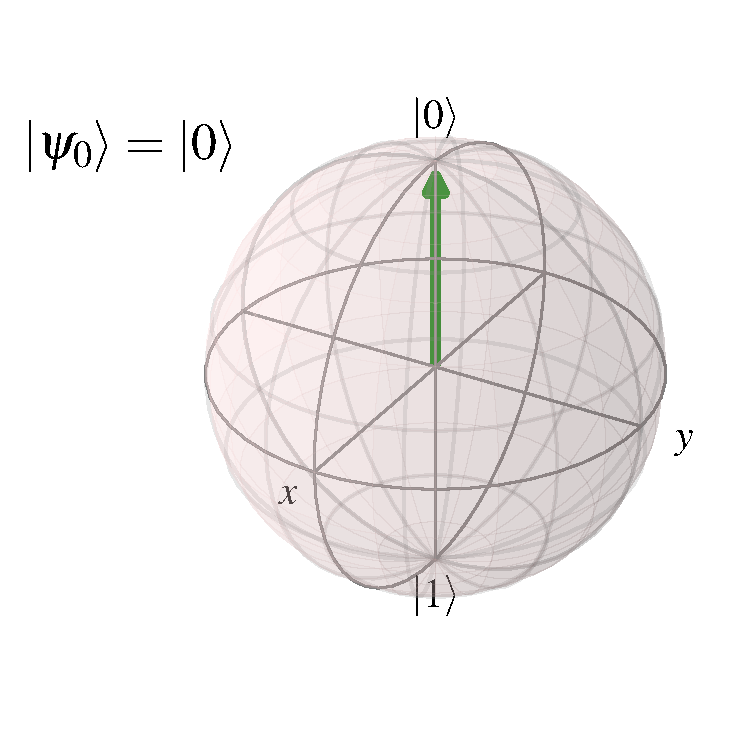
\includegraphics[width=0.2\textwidth]{experimental_study/figures/hahn_bloch_spheres/bloch_0.pdf}
        }
        \qquad
        \subfloat{
            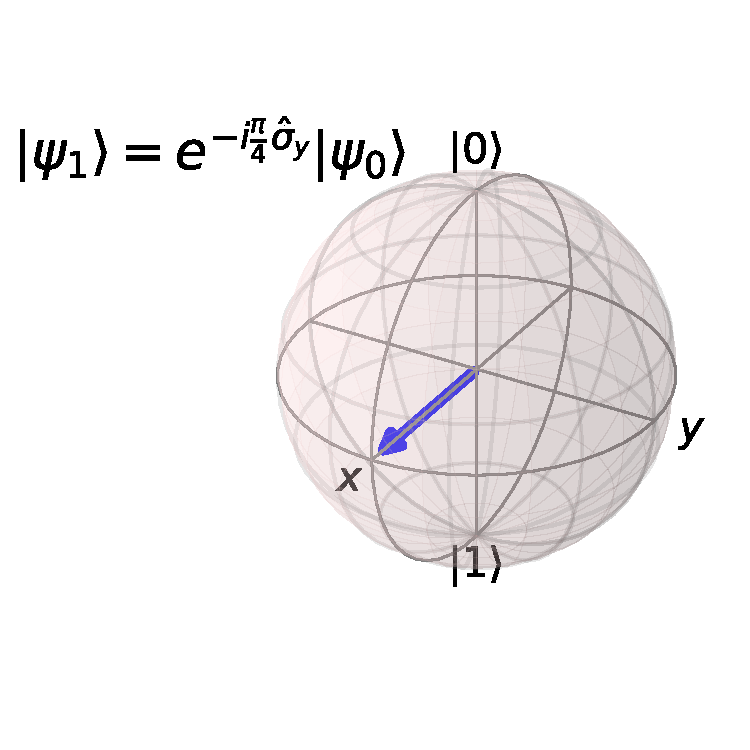
\includegraphics[width=0.2\textwidth]{experimental_study/figures/hahn_bloch_spheres/bloch_1.pdf}
        }
        \qquad
        \subfloat{
            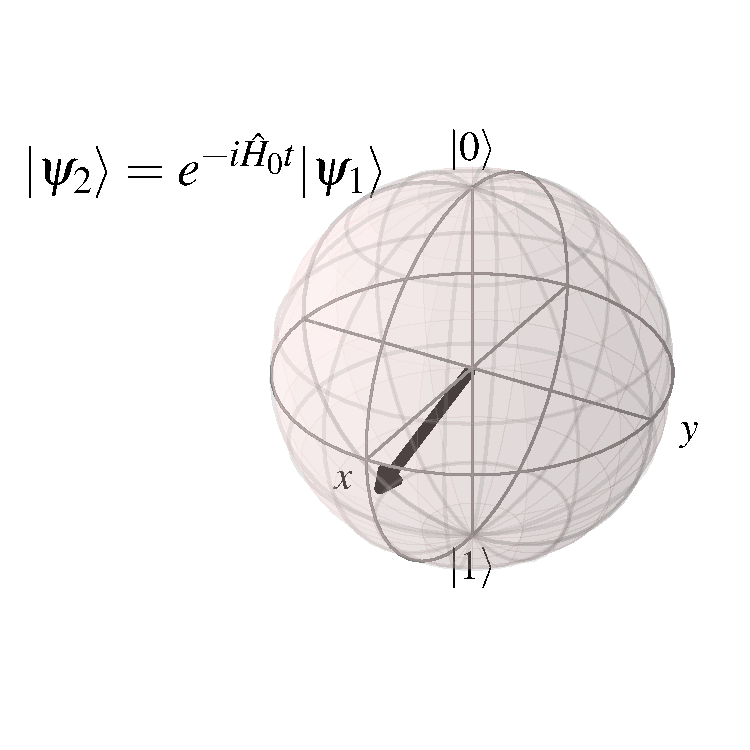
\includegraphics[width=0.2\textwidth]{experimental_study/figures/hahn_bloch_spheres/bloch_2.pdf}
        }
        \\
        \qquad
        \subfloat{
            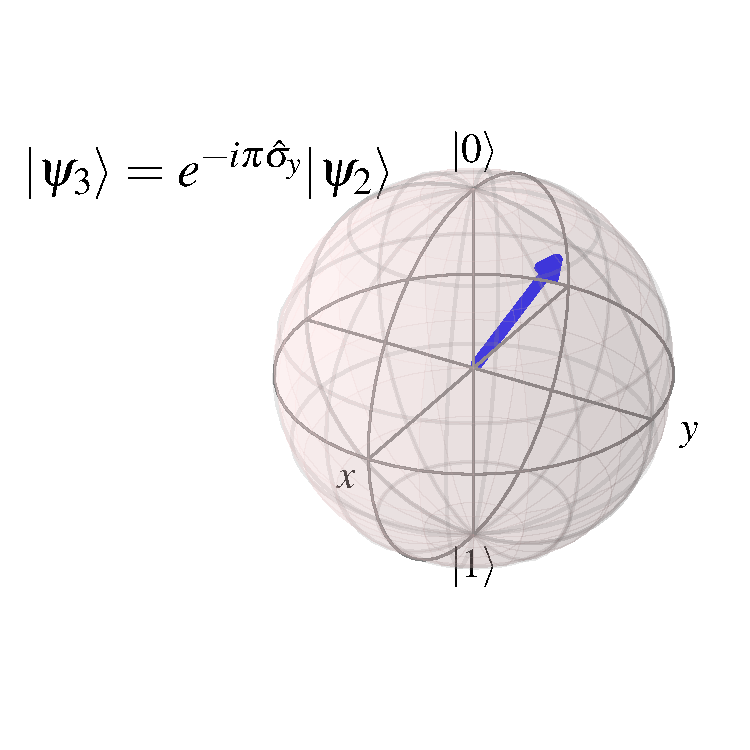
\includegraphics[width=0.2\textwidth]{experimental_study/figures/hahn_bloch_spheres/bloch_3.pdf}
        }
        \qquad
        \subfloat{
            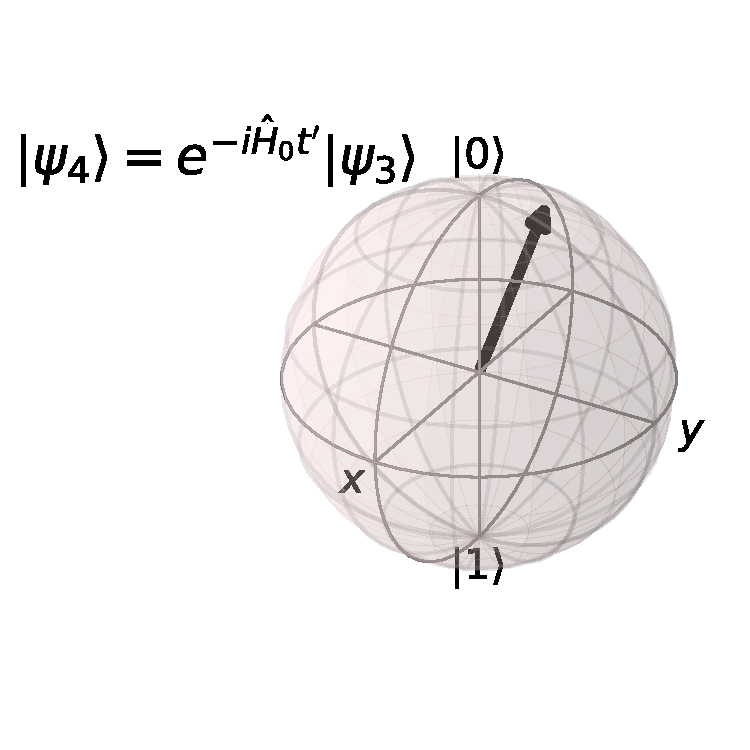
\includegraphics[width=0.2\textwidth]{experimental_study/figures/hahn_bloch_spheres/bloch_4.pdf}
        }
        \qquad
        \subfloat{
            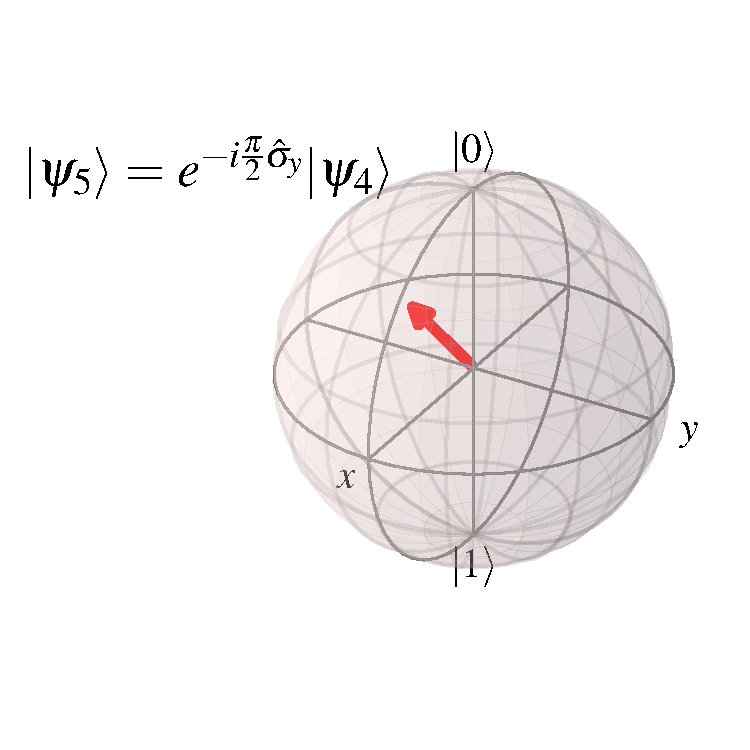
\includegraphics[width=0.2\textwidth]{experimental_study/figures/hahn_bloch_spheres/bloch_5.pdf}
        }
    \end{center}
    \caption[States of spin qubit at each stage of Hahn echo sequence]{
        States of spin qubit at each stage of Hahn echo sequence.
        
        The state of the \gls{nvc} spin is initialised by a green laser into state $\ket{\psi_0} = \ket{0}$. 
        We then apply a rotation about the $y$-axis (i.e. a \gls{mw} pulse), 
            yielding the state $\ket{\psi_1} = \ket{+}$. 
        The system is then allowed to evolve according to its own $\ho$ for $t$, $\ket{\psi_2} = e^{-i\ho t}\ket{+}$.
        We apply a second \gls{mw} pulse, this time for a $\pi$-rotation about the $y$-axis, 
        $\ket{\psi_3} = e^{-i\pi \s_y}e^{-i\ho t}\ket{+}$.
        Again the system evolves according to interactions with the environment, this time for $t^{\prime} = 2t$.
        We apply a final \gls{mw} pulse to rotate about the $y$-axis again, 
            effectively either returning the spin to near the $\ket{0}$ axis, 
            or near the $\ket{1}$ axis. 
        Here $\ket{\psi_5}$ is roughly half way between $\ket{0}$ and $\ket{+}$, 
        i.e. along the $z$-axis. 
        The spin is read out from $\ket{\psi_5}$ via the \gls{nvc}'s \glsentrylong{pl}. 
        Here $\ho = 0.25 \ \s_y$ was evolved for $t=0.5$ (arbitrary units), 
        and the final state overlap with the initial state, 
        i.e. the likelihood of measuring the spin in $\ket{0}$ is $\Pr(0 | \ho, t) = 0.865$. 
    }
    \label{fig:hahn_bloch_spheres}
\end{figure}
    
We have decided to characterise the hyperfine interactions of the \gls{nvc}; 
    these are evident most strongly at very short timescales \cite{childress2006coherent}. 
To isolate the effects of the hyperfine interactions, 
    we run Hahn echo experiments, which are known to emphasise weak interactions.
Hahn echo sequences attempt to decouple the spin's dynamics from the nuclear bath
    \cite{rowan1965electron, blok2014manipulating, childress2006coherent, charnock2001combined, gentile2020Operating}
    providing a helpful platform for studying residual contributions of terms in \cref{eqn:nv_terms}.
The \gls{nvc} qubit undergoes a series of evolutions -- either according to application of quantum logic gates
    or the natural evolution of the system interacting with its environmen  
We depict the stages of the experiment in \cref{fig:hahn_bloch_spheres}, 
    starting from the initialised $\ket{0}$
    through to its final state which is read out through \gls{pl},
    both of which as described in \cref{sec:nv_centres}.
\par 

In particular, the final state, $\ket{\psi}_5$, is read out, effectively by projection onto $\ket{0}$;
    we can interpret the \gls{pl} after evolution time $t$ as the \gls{likelihood} 
    that the \gls{nvc} is found in $\ket{0}$ after evolution of its \emph{true} Hamiltonian, $\ho$. 
That is, we assign this projection as the quantity $\Pr(0 | \ho, t)$ (the \gls{likelihood}), 
    and it can be used within likelihood estimation in order to refine a candidate model $\hj$, 
    effectively\footnotemark \ by changing the structure of 
    $\hj$ until $\Pr(0 | \ho, t) \approx \Pr(0 | \hj, t) \ \forall t$. 

\footnotetext{
    Of course this is a gross simplification of \gls{qhl} which is described fully in \cref{sec:qhl}
}
\par 

By varying the evolution time of the Hahn-echo sequence, we can map the likelihood 
    against time, which we can view as capturing the dynamics of the \gls{nvc} spin \cref{fig:exp_raw_data}.
We vary time up to $t \sim 4 \mu s$ in the short-time range in intervals of $\Delta t = 50 ns$, 
    so we have 425 data points. 
Importantly, the data for the studied \gls{nvc} is taken once and analysed offline, 
    i.e. \gls{qmla} does not have complete authority to design experiments 
    to run on the \gls{nvc}, although it can aim to choose the most informative $t$ 
    available in the predefined set; we will discuss the consequences of this restriction 
    later in this chapter. 

\begin{figure}
    \begin{center}
        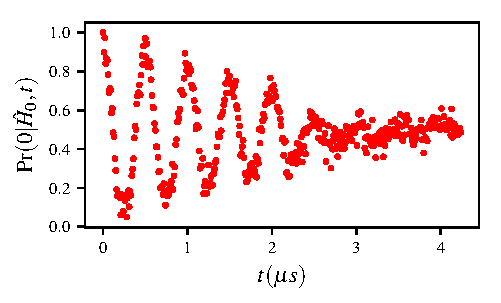
\includegraphics{experimental_study/figures/raw_data.pdf}
    \end{center}
    \caption[Raw data for \glsentrylong{nvc}'s dynamics]{
        Raw data for the \glsentrylong{nvc}'s dynamics.
        The $y$-axis shows the \glsentrylong{pl} of the \gls{nvc}, 
        equivalently the likelihood $\Pr(0 | \ho, t)$. 
    }
    \label{fig:nv_raw_data}
\end{figure}


\section{\Glsentrylong{es}}\label{sec:exp_es}
Finally, then, we are in a position to describe the specific implementation details 
    which allow \gls{qmla} to study this \gls{nvc} system. 
Recalling the terminology of \gls{qmla} from \cref{chapter:qmla}, 
    we design an \glsentryfull{es} specifically for the system under study. 
The \gls{es} will account for the details listed in this chapter so far, in summary: 
\begin{easylist}[itemize]
    & we attempt to assign a model, $\hp$, to the \gls{nvc};
    && we especially focus on its hyperfine interactions;
    & in particular, we use a 2-qubit approximation;
    && the first qubit represent the spin itself;
    && the second qubit represents the environment in which the \gls{nvc} resides;
    & we query the \gls{nvc} by performing Hahn echo experiments (\cref{fig:hahn_bloch_spheres});
    & the outcome of those experiments are thought of as the system's likelihoods (\cref{fig:nv_raw_data});
    & likelihoods are used for the training of individual candidate models;
    & candidate models are composed of the terms defined in \cref{eqn:nv_terms}.
\end{easylist}   
\par 

As outlined in \cref{sec:exploration_strategies}, the central role of any \gls{es} is to specify the 
    model generation procedure, which \gls{qmla} relies upon for deciding the next set of candidate models to test. 
In this case, we exploit some intuition and prior knowledge of how such systems work, 
    to design a bespoke model generation subroutine:
    we can think of this as a midway point between the completely specified \glspl{es} used 
    for identifying the underlying lattices from a prescribed set in \cref{chapter:lattices}, 
    and the entirely general \glsentrylong{ga} which does not restrict model generation, of \cref{chapter:ga}.
We use the standart structure of \glspl{et} introduced in \cref{sec:exploration_strategies}, 
    where models are placed on consecutive branches, $\mu$, with branches consolidated by complete pairwise 
    comparisons, mediated through \glspl{bf}, resulting in the selection of a single branch champion, $\hat{H}_{C(\mu)}$. 
\par 


\begin{figure}
    \begin{center}
        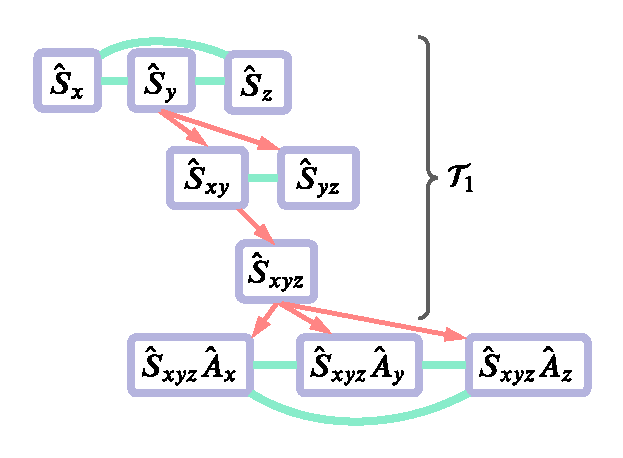
\includegraphics[width=0.5\textwidth]{experimental_study/figures/greedy_search.pdf}
    \end{center}
    \caption[Greedy model search]{
        Greedy model search. 
        Models (purple) are placed on branches, trained and consolidated (green) as in \cref{fig:qmla_overview}, 
            with the branch champion spawning (red) candidates to place on the subsequent branch.  
        Branches are grouped in tiers, correspdoning to levels of approximation:
            the first tier of the model generation strategy is shown, 
            where $\termset_1 = \{ \hat{S}_x, \hat{S}_y, \hat{S}_z\}$ is explored. 
        The final champion from the first tier seeds the second tier. 
    }
    \label{fig:greedy_search}
\end{figure}

We use a \emph{greedy search rule}: 
    terms are added one-by-one to gradually increase the complexity of candidate models until terms are exhausted \cite{russell2002artificial}.  
We break the \gls{et} into three distinct tiers, each corresponding to an intuitive degree of complexity:
    the first tier involves the spin-only terms, $\termset_1 = \{ \hat{S}_i \}$; 
    the second considers the hyperfine terms, $\termset_2 = \{ \hat{A}_i \}$;
    the final tier the transverse terms, $\termset_3 = \{ \hat{T}_i\}$.  
Within each tier, terms are added greedily to the previous branch's champion, $\hat{H}_{C(\mu)}$.
So, the first branch is given by $\mu = \{ \hat{S}_x, \hat{S}_y, \hat{S}_z\}$;
    say $\hat{H}_{C(\mu)} = \hat{S}_y$, then $\mu + 1$  determines that $\hat{S}_x, \hat{S}_z$ 
    are not yet considerd, so it constructs the models $\hat{S}_{x,y}, \hat{S}_{y,z}$, e.g. \cref{fig:greedy_search}. 
After exhausting all tiers, we consolidate the set of branch champions, $\mathbb{H}_C = \{ \h_{C(\mu)}\}$, 
    to determine the best model considered globally, $\hp$.  
\par 
Clearly, this growth rule is partially deterministic, insofar as some models are gauranteed to be considered, 
    while others are not reachable; 
    indeed, the space of available models are heavily constrained, in particular models in later tiers will 
    always involve all of the tier 1 models, e.g. $\hat{S}_{x}\hat{A}_{y}$ does not occur naturally. 
We account for this shortcoming with a final redcibility test, 
    triggered if any of the parameters of $\hp$ are potentially negligible, 
    i.e. are within one standard deviation of 0. 
This test simply removes such low-parmeter terms from $\hp$, 
    giving a reduced global champion, $\hp_r$, 
    and computes the \gls{bf} between $\hp, \hp_r$: 
    if the \gls{bf} indicates strong evidence in favour of the reduced version, 
    we replace the champion model, $\hp \gets \hp_r$. 
In effect, we thus verify the statistical significance of each term included in $\hp$. 
\par 

The total model in \cref{eqn:nv_ham_full} supports $N_t = 1 + 3 + 6 | \chi | + 3 + 3 |\chi| = 7 + 9|\chi| $ terms, 
    which we reduced to a space of $N_t=3 + 6 |\chi| = 9$ through several approximations\footenotemark ;
    even so, the remainng $2^9$ permitted models were reduced further by building the logic of this \gls{es} 
    from our intuition aroud existing knowledge of typical \gls{nvc} systems,
    such the \gls{es} will only ever consider $<20$ models per instance. 
The described \gls{es} seems overly perscriptive, 
    but should be viewed as a first attempt at a generalisable approach: 
    essentially we can view the tiers of the greedy search as characterising the system 
    at various approximations, 
    e.g. the first tier examines one-qubit terms, while subsequent tiers inspect $2$-qubit terms. 
We can envision future work where the greedy search is gradually extended to less rigid approximations, 
    enabling study of more complex quantum systems.     
This leads to some important remarks:

\begin{easylist}[enumerate]
    \ListProperties()
    & Realistic, near-term applications of \gls{qmla} can not be thought of as a solution to black-box characterisation problems: 
        it must be used in conjunction with domain expertise for the system under study.
    & While this test-case yields promising results, the outcome of \gls{qmla} here may not be especially insightful, 
        since the available model terms were so deliberately constrained -- we demonstrate a use-case in \cref{chapter:many_qubits} 
        where a broader scope is enabled in simulation.    
\end{easylist}   
\par 

A common charge against \gls{qmla} supposes to first write down the most complex model, 
    train it fully, and then infer which terms are negligible, in a similar process to the champion reduction test outlined here. 
While this may be feasible in the case described here, with $N_t=9$ and a closed term set, 
    this would scale poorly: adding just a second nuclear site increases the model search to a space of $N_t=15$.
Models of higher cardinality ($|\al|$) demand higher $\Ne, \Np$ to train well, so immediately trainng the most involved model would 
    require infeasible resources\footnotemark, and risks significantly overfitting the data. 
It seems more appropriate to work ``from the ground up'', testing terms and keeping them only when justified, 
    instead of training all terms and attempting to decouple their effects post-hoc. 

\footnotetext{
    Note: in the case studies presented in this thesis, it was found that the same resources were sufficient for the simplest and most complex models, 
    due to the relatively small number of terms therein.
    We expect for larger models, e.g. $|\al|>10$, that the resources allocated ought to be proportional to the cardinality, 
    which is an in-built option in the \gls{qmla} software. 
}
\par 
\subsection{Test in simulation}
Before considering the real experimental data (\cref{fig:nv_raw_data}), 
    we first test the \gls{es} in simulation under ideal conditions. 
That is, we assume the ability to prepare arbitrary probe states, 
    and use a random probe set (see \cref{sec:probes}),
    and use the full expectation value as the likelihood, $|\braket{\psi | e^{-i \hj t} | \psi}|^2$.
Of course, this is infeasible since we presume access to the full state at the time of measurement, 
    but this can be seen as a best-case scenario for this application, 
    because the realistic case loses information by tracing out the environmental qubit at measurement.
We vary the target $\ho$, among a series of ten models,
    which are all valid models achievable by the \gls{es}. 

Varying $\ho$, allowing arbitrary probe preparation and \gls{pgh} \gls{edh}, 
    i.e. case (i) from \cite{gentile2020learning}. 

\section{Experiment design constraints}
Moving to analyse the experimental setup, there are a number of constraints which we must account for in 
    training models. 
Firstly, the $\nicefrac{\pi}{2}$-pulse applied to the prepared qubit ($\ket{\psi_0} \rightarrow \ket{\psi_1}$ in \cref{fig:hahn_bloch_spheres})
    means that the state before evolution is always $\ket{+}$ in the computational basis;
    this is a severe limitation on model training, as we saw in \cref{sec:probes}. 
Moreover, this puts a bias on the interactions \gls{qmla} is likely to identify:
    we show in \cref{fig:hahn_bloch_spheres} how \gls{qhl} performs in training the same model using 
    (i) the probe set available experimentally; (ii) a more general (random) probe set. 
This has a noteworthy impact on the outcome of this study, 
    since this suppression of terms means we are more likely to find some interactions
    than others, so we must add this caveat to the champion model. 
\par

The experiment was run until the \gls{nvc} was deemed to have decohered, 
    so \cref{fig:nv_raw_data} ceases at $t_{\textrm{max}} \sim \ 4 \mu s$. 
As discussed in \cref{sec:edh}, usually it is helpful to allow a \glsentryfull{edh} to
    choose the experimental controls, including the evoltuion time, $t$, against which 
    the model is trained at each experiment;
    the default \glsentryfull{pgh} attempts to select $t$ at the upper boundary of times 
    where the model is expected to be predictive, such as to maximise the information gained by the experiment (see \cref{sec:pgh}). 
Here, however, we can not allow the \gls{edh} to select arbitrary $t$, 
    since we do not have data beyond $t_{\textrm{max}}$. 

\par 

Clearly, we require a custom \gls{edh} to account for the constraints outlined, 
    with the following considerations: 
\begin{easylist}[enumerate]
    & We may only assume access to the probe $\ket{+}$ on the spin qubit
    && we further assume the environmental spin is polarised by the same microwave pulse, 
        such that the global probe available is $\ket{\psi} = \ket{+}\ket{+^{\prime}}$, with 
        $\ket{+^{\prime}} = \frac{\ket{0} + e^{i \phi} \ket{1}}{\sqrt{2}}$ and $\phi$ is random \cite{broadway2018quantum}. 
    & We can not allow the choice of any $t$
    && Any $t > t_{\textrm{max}}$, arising from a thin parameter distribution, 
        must be mapped to some $0 < t \leq t_{\textrm{max}}$. 
    && All nominated $t$ must be mapped to the nearest available $t$ in the dataset
        so that the likelihoods are as close as possible to simulating the true system. 
    & Much of the physics of interest occurs at relatively high times, 
        i.e. because the rotation ($\mhz$) terms dominate, the decay of the peaks
        can be seen as evidence of the bath, notably through hyperfine terms in the model. 
    && We therefore wish to enforce that all models are trained on those data ($t \geq 2 \mu s)$,
        even if their parameter distribution is insufficiently narrow to yield those times naturally. 
\end{easylist}

Accounting for these, we construct an \gls{edh} which mixes the robust, adaptive nature of \gls{pgh}, 
    useful for refining an initially broad $\Pr(\al)$,
    with a primitive, linear time-selection, useful to ensure the trained parameters at least
    attempt to account for the physics we are actually interested in. 
That is, with each model trained for $\Ne$ experiments, 
    we train according to the standard \gls{pgh} for the first $\nicefrac{\Ne}{2}$, 
    but force the training to mediate over the available data for the latter $\nicefrac{\Ne}{2}$. 
\par 

\section{Results}
\begin{table}[h]
    \centering
    \begin{tabular}{cllrr}
    \hline
     Model & \multicolumn{2}{c}{Experiment} & \multicolumn{2}{c}{Simulation}    \\
     & Wins   & $R^2$   & Wins   & $R^2$   \\
    \hline
    \\
     $\hat{S}_{y,z}\hat{A}_{z}$                      & 9      & 0.8     & 1      & 0.26    \\
     $\hat{S}_{y}\hat{A}_{x,z}$                      & 2      & 0.63    &        &         \\
     $\hat{S}_{x,y,z}\hat{A}_{z}$                    & 45     & 0.86    & 61     & 0.97    \\
     $\hat{S}_{x,y,z}\hat{A}_{y}$                    &        &         & 1      & -0.54   \\
     $\hat{S}_{x,y,z}\hat{A}_{x,y}$                  & 3      & 0.81    &        &         \\
     $\hat{S}_{x,y,z}\hat{A}_{y,z}$                  & 14     & 0.83    & 10     & 0.96    \\
     $\hat{S}_{x,y,z}\hat{A}_{x,z}$                  & 6      & 0.64    & 15     & 0.99    \\
     $\hat{S}_{x,y,z}\hat{A}_{x,y,z}$                & 2      & 0.72    & 5      & 0.97    \\
     $\hat{S}_{x,y,z}\hat{A}_{x,z}\hat{T}_{xz}$      &        &         & 1      & 0.68    \\
     $\hat{S}_{x,y,z}\hat{A}_{x,y,z}\hat{T}_{xz}$    &        &         & 5      & 0.77    \\
     $\hat{S}_{y}\hat{A}_{x,y,z}\hat{T}_{xy,xz,yz}$  & 2      & 0.31    &        &         \\
     $\hat{S}_{x,y,z}\hat{A}_{x,y,z}\hat{T}_{xy,xz}$ & 4      & 0.67    & 1      & 0.32    \\
    \hline
    \end{tabular}
    \caption[
        \gls{qmla} win rates and $R^2$ for models based on experimental data and simulations. 
    ]{
        \gls{qmla} win rates and $R^2$ for models based on experimental data and simulations. 
        We state the number of \gls{qmla} instances won by each model and the average $R^2$ for those instances as an indication of the
        predictive power of winning models.
    }
    \label{table:win_rates_r_squareds}
\end{table}

We apply the \gls{es} described in \cref{sec:exp_es} to the raw data of \cref{fig:nv_raw_data};
    the results are summarised in \cref{fig:exp_qmla_analysis}.
\par 

We first focus on the overall outcomes:
    the most blunt figure of merit of interest is simply whether \gls{qmla}
    overfits or underits the true parameterisation. 
In preliminary analysis we run 500 instances with varying $\ho$, 
    and where the cardinality of $\ho$ ranges,
    so we can broadly gauge the tendency towards over- and under-fitting:
    we see that in $\sim~50\%$ of instances the correct cardinality is found,  
    rising to $\sim~86\%$ by allowing one fewer (additional) terms, \cref{fig:exp_qmla_analysis}\textbf{(b)}. 
Moreover, the champion models' are highly predictive: 
    the median coefficient of determination between the systems' and corresponding champion models' data is 
    $R^2 = 0.84$. 
\par 

\begin{figure}
    \includegraphics[width=0.95\textwidth]{experimental_study/figures/experimental_qmla_analysis.pdf}
    \caption[\gls{qmla} applied to experimental \glsentrylong{nvc} system]{
        \textbf{a}, 
        The carbon lattice providing the outer environment for the NV centre, along with the
        time evolution of the electron spin state (represented on a Bloch sphere) during the pulses for the Hahn-echo sequences. The final $\pi/2$ pulse is omitted.  
        \textbf{b}, 
        Simulation of 500 independent \gls{qmla} instances, where $\ho$ is chosen randomly. 
        The win rate is reported against the difference $(N_{p}-N^{\prime}_p)$ between the 
        number of parameters in $\hp$ and $\ho$, respectively. 
        The \emph{under-parameterised} \emph{ (over-parameterised)} class refers to models with less (more) 
        parameters than $\ho$. 
        \emph{Correct} indicates that exactly $\ho$ was found. 
        The \emph{mis-parameterised} class groups models with the same parametrisation cardinality as $\ho$, but different Hamiltonian terms. 
        \textbf{Inset}, Histogram of occurrences of $R^2$ values for each retrieved $\hp$ 
        against a sampling of datapoints from $\ho$, with median $R^2=0.84$ (red dotted line). 
        \textbf{c}, 
        Win rates of top four models for 100 \gls{qmla} instances, 
        against both simulated and experimental data. 
        Simulations use $\ho = \SxyzAz$.
        \textbf{d}, 
        Total volume spanned by the parameters' prior across epochs, for the models in \textbf{c}. 
        Shaded areas indicate $66\%$ credible regions. 
        \textbf{e}, 
        Simulated likelihoods reproduced by the model with the highest win rate ($\hat{S}_{x,y,z}\hat{A}_{z}$, turquoise), 
            compared with corresponding NV-centre system experimental data (
                red-dots, extracted from the observed \gls{pl} of the first Hahn-echo decay). 
        Error bars smaller than the dots (see Methods).
        \textbf{f}, 
        A single QMLA instance against experimental data in \textbf{e}, depicted as a \gls{dag}.
        The thin end of each edge points to the favoured model; 
        the colour of the edges maps $\log_{10}\mathcal{B}$ as in the bar legend at the bottom. 
        Layer champions \huc are in light brown, whereas the global champion $\hp$  is in orange.    
    }
    \label{fig:exp_qmla_analysis}
\end{figure}
Then, considering the performance of the algorithm on whole, 
    we perform \glspl{run} of 100 instances on the exerpimental data as well as simulated data,
    where the simulation assumes\footnotemark \ $\ho = \hat{S}_{xyz} \hat{A}_z$, 
    The set of models selected most frequently are shown in \cref{fig:exp_qmla_analysis}\textbf{(c)},
    and each model is trained with $\Ne=1000, \Np=3000$,
    with the \glspl{volume} of those models (in the experimental case) shown in  \cref{fig:exp_qmla_analysis}\textbf{(d)}.
\footnotetext{
    Here we work backwards by setting the target model as that which \gls{qmla} deemed most appropriate for the available data.
    We posit that this choice is arbitrary and doesn't fundamentally change the discussion of this chapter, 
    merely aiding in analysing the performance of the algorithm with respect to a concrete example.
}
In particular, the most prominent models, $\{ \SxyzAz, \SxyzAyz, \SxyzAxz, \SyzAz \}$ are found collectively in 74\% (87\%)
    of instances on the experimental (simulated) data;
    the win rates and $R^2$ of all models (which won at least one instance) are reported in \cref{table:win_rates_r_squareds}. 
It is noteworthy that even in the simulated case, the same models mislead \gls{qmla}:
    this suggests that the resultant physics from these models is substantially similar to that of the true model\footnotemark. 
\footnotetext{Alternatively, that the same systematic error misdirects the search in both cases.}
These models are defensible with respect to the descriptions of \cref{sec:target_system}, 
    since in each case they detect the interaction between the spin qubit and the environmental qubit, 
    i.e. the hyperfine terms $\hat{A}_i$, especially $\hat{A}_z$ which occurs in 97\% (99\%) of champions. 
We discuss some physical insights from these results in \cref{sec:exp_qmla_analysis}.   
\par 



The most frequently found model, $\hp = \SxyzAz$, is found in $45\%$ ($61\%$) of instances:
    we show its attempt to reproduce the dynamics of \cref{fig:nv_raw_data} in \cref{fig:exp_qmla_analysis}\textbf{(e)}, 
    showing excellent agreement with the raw data, with $R^2=0.82$. 
This serves as an essential sanity check: 
    we can intuitively see that \gls{qmla} has distilled a model which captures at least \emph{some} 
    of the most important physical interactions the target \gls{nvc} system is subject to; 
    otherwise we would not see such clear overlap between the prediced and true dynamics. 
\par 

Finally we display the model search as a \gls{dag} in \cref{fig:exp_qmla_analysis}\textbf{(f)}, 
    where models are represented on nodes on the graphs layers (equivalent to \gls{et} branches), 
    and their parents are resident on the branch immediately above their own.
Comparisons between models, $\hi, \hj$,  are shown as edges between nodes on the graph, 
    coloured by the strength of evidence of the outcome, the \gls{bf}, $\bij$. 
Each layer, $\mu$, nominates their branch champion, $\hat{H}_{C(\mu)}$;
    the set of branch champions are consolidated to determine the global champion, $\hp_C$. 
\subsection{Analysis}\label{sec:exp_qmla_analysis}


\begin{figure}
    \begin{center}
        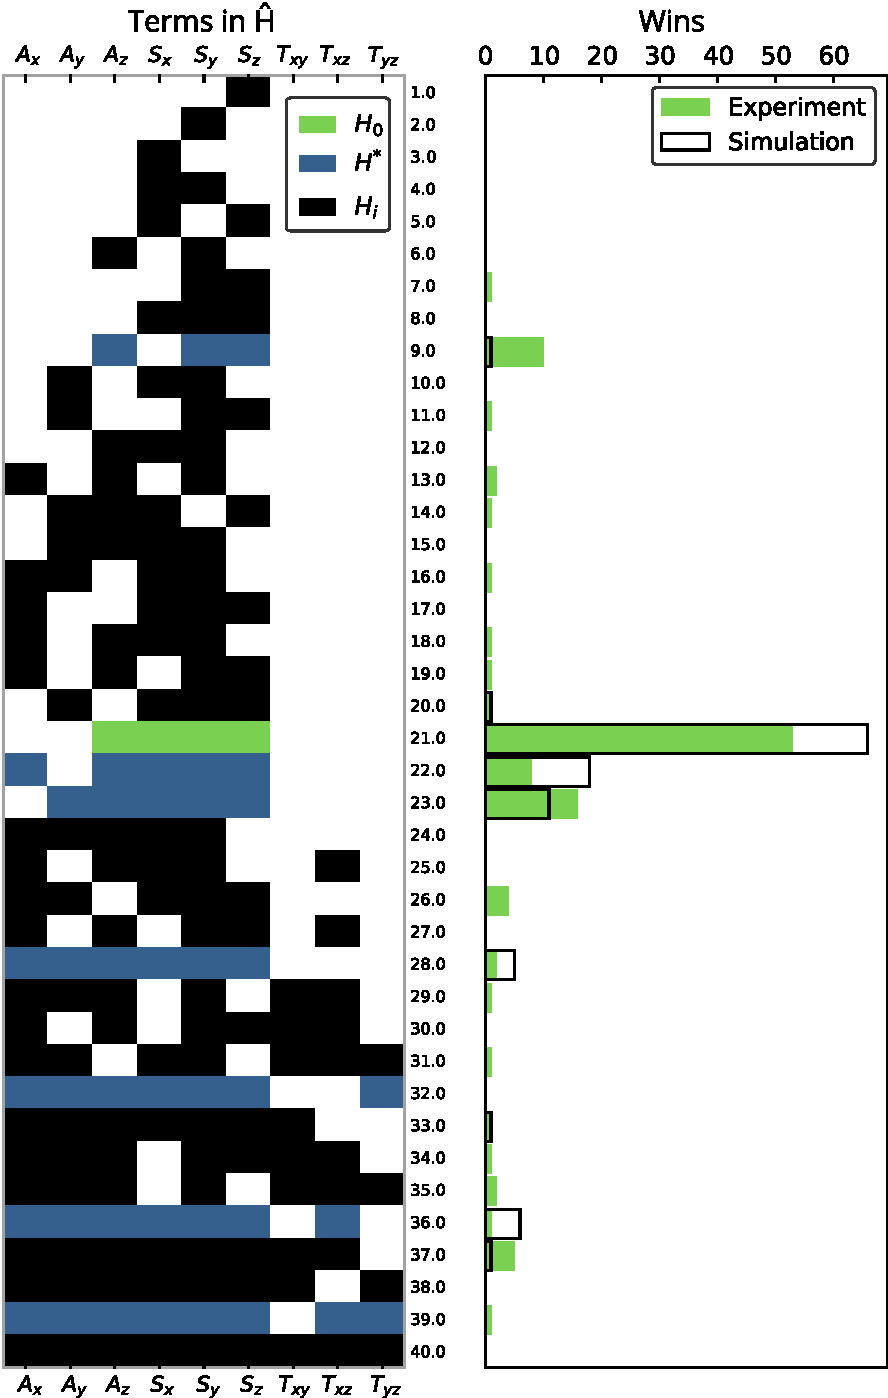
\includegraphics[width=0.6\textwidth]{experimental_study/figures/model_composition.pdf}
    \end{center}
    \caption[
        Models considered by \gls{qmla} for simulated/experimental \glsentrylong{nvc} data, and their win rates
    ]{
    \textbf{Left}: map of the various Hamiltonian terms included in each of the possible 40 candidate models explored by \gls{qmla}
    during any of the 100 instances on either simulated or experimental data.
    The explicit form of each operator can be inferred from \cref{win_rates_r_squareds}.
    IDs of candidate models are on the vertical axis, and labels for the terms on the horizontal axis.
    The true model $\hat{H}_0$ for the simulated case is highlighted in green and a subset of credible models in blue, 
    i.e. models which may reasonbaly be expected to describe the \gls{nvc} from theoretical arguments.
    \textbf{Right}: wins for each of the candidate models as above out of $100$ independent QMLA runs, 
    reported as a histogram for cases adopting simulated data (empty bars) or the experimental dataset.
    } 
    \label{fig:nv_model_composition}
    % /home/bf16951/Dropbox/QML_share_stateofart/PAPER/Figures/SuppMat/multi_instance_analysis notebook
\end{figure}

Considering the \glspl{run} summarised in \cref{fig:exp_qmla_analysis}, here we will present some furhter perspecitives.
\cref{fig:nv_model_composition} first details all models considered in the 200 \glspl{instance} 
    comprising the experimental and simulated \gls{qmla} \glspl{run}, 
    as well as the win rate of each model. 
This \gls{es} is designed to study a small subspace of the overall available space:
    only $40$ unique models are constructed. 
We highlight a number of \emph{credible} models which we deem especially valid approximations of the target system, 
    i.e. which contain the most viable approximations. 
\par 

\begin{figure}
    \centering
    \begin{tabular}{@{}c@{}}
        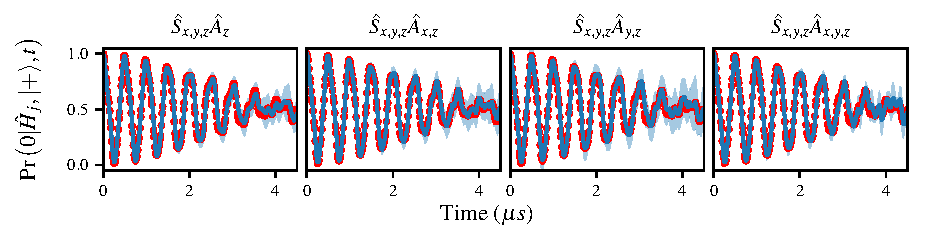
\includegraphics{experimental_study/figures/reproduced_dyamics_sim.pdf}
    \end{tabular}
    \\ \small \textbf{a,} Simulated data
    \centering

    \begin{tabular}{@{}c@{}}
        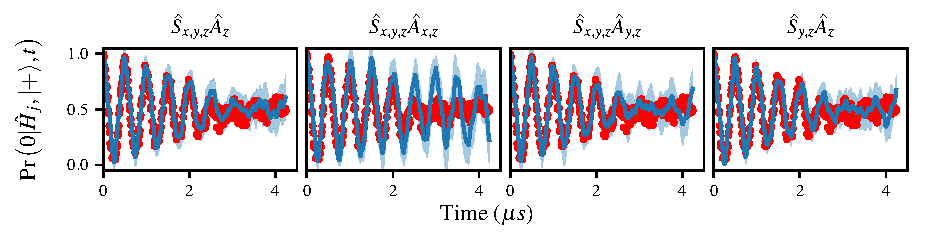
\includegraphics{experimental_study/figures/reproduced_dyamics_exp.pdf}
    \end{tabular}
    \\ \small \textbf{b,} Experimental data

    \caption[Dynamics reproduced by \gls{qmla} champion models for simulated/experimental data]{
        Dynamics reproduced by various \gls{qmla} champion models for simulated/experimental data. 
        Expectation values are shown on $y$--axis with time on $x$--axis. 
        Red dots give the true dynamics of $\ho$, while the blue lines show the median reconstruction by $\hp$
        from all the instance where that model was deemed $\hp$, with light blue showing the standard deviation of those likelihoods.   
        $\hp$ \ is listed on top of each plot; the number of instances won by each model can be read from \cref{table:win_rates_r_squareds}. 
    
    }
    \label{fig:nv_model_dynamics}
    % figure_development/nv_dynamics_reproduction.ipynb
\end{figure}

\cref{fig:nv_model_dynamics} shows the reproduction of dynamics of the top four models
    from both simulated and experimental \glspl{run}. 
We see that each model faithfully captures the essential dynamics arising from the respective target systems;
    this alone is insufficient to conclude that the true model has been identified, 
    but serves as a valuable \emph{sanity-check}, convincing us that the output of \gls{qmla} is at least a sensible 
    approximation of $\ho$, if not the absolutely true model.
\par 


\begin{figure}
    \centering
    \begin{tabular}{@{}c@{}}
        \centering
        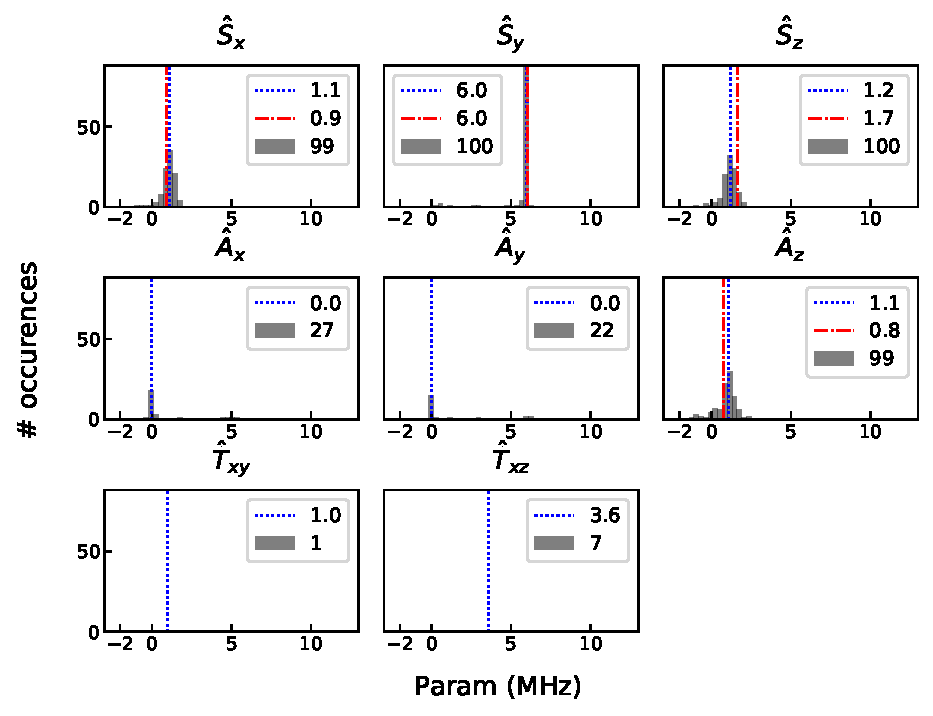
\includegraphics[width=0.7\textwidth]{experimental_study/figures/params_simulation.pdf}
    \end{tabular}
    \\ \small \textbf{a,} Simluated QMLA instances. Red dotted lines show the true parameters.
    
    \centering
    \begin{tabular}{@{}c@{}}
        \centering
        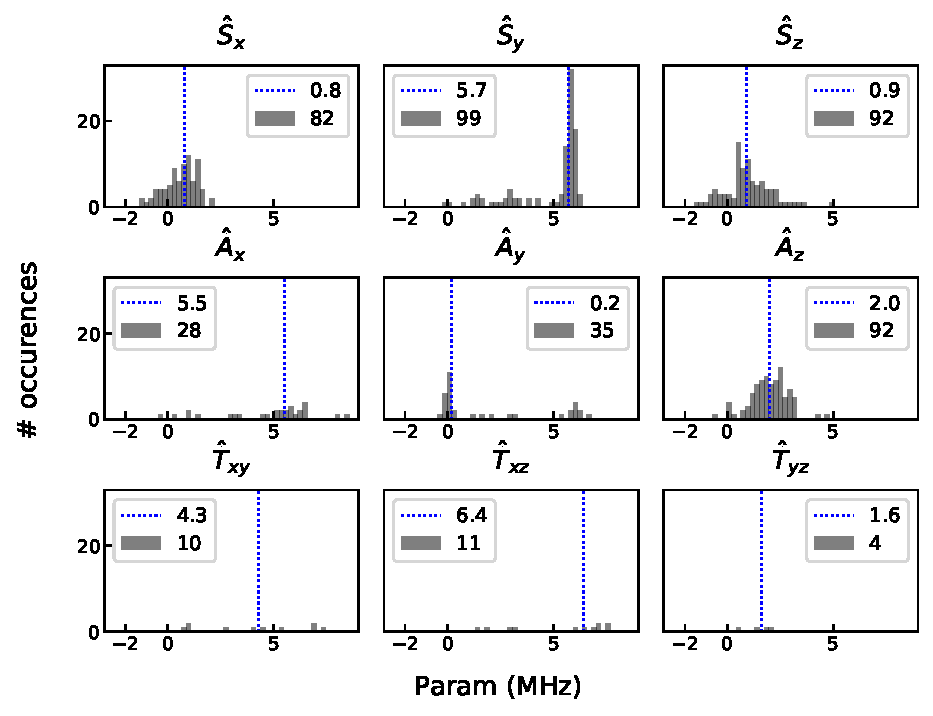
\includegraphics[width=0.7\textwidth]{experimental_study/figures/params_experimental.pdf}
    \end{tabular}
    \\
    \small \textbf{b,} Experimental QMLA instances.
    % \centerline \small \textbf{b,} Experimental QMLA instances.
    \caption[
        Histograms for parameters learned by \gls{qmla} champion models on simulated and experimental data
    ]{
        Histograms for parameters learned by \gls{qmla} champion models on (\textbf{a}) simulated  and (\textbf{b}) experimental data. 
        Blue dotted lines indicate the median for that parameter; grey blocks show the number of models which found the parameter
        to have that value and the number listed in the legend reports how many champion models contained that term.
    }
    \label{fig:nv_learned_params}
    % /home/bf16951/Dropbox/QML_share_stateofart/Auxiliary files/QMLA plots via pandas
\end{figure}

The key insight promised by \gls{qmla} is to identfiy the interactions present in the studied system. 
In \cref{fig:nv_learned_params} we show the number of times each of the terms permitted (\cref{eqn:nv_terms})
    is included in the champion model; 
    we also show the distribution of parameter estimates for those terms. 
From the simulated case, we see that those terms which are in $\ho$, i.e. $\termset_0$, are found in almost all instances; 
    furthermore, while some terms are erroneoulsy found in $>40\%$ of instances, 
    they are found with less than a quarter of the frequency of the true terms,
    so these may be reasonably ruled out in post-processing the \gls{qmla} results. 
The inaccurate terms found most often are seen to have (almost) negligible parameters:
    in conjunction with domain expertise, users can determine whether the inclusion of these terms 
    are meaningful or simply artefacts of slight overfitting.
In the experimental \gls{run}, on the other hand, we see a similar gulf in frequency between some terms.
Namely, $\{ \hat{S}_x, \hat{S}_y, \hat{S}_z, \hat{A}_z \}$ are found in $50+$ more instances than all others:
    we therefore conclude that those terms contribute most strongly to the \gls{nvc}.
The parameters found for these terms are of the same order of magnitude as we would have predicted originally, 
    but disagreee in the precise value. 
For example, the rotation about the $y$-axis, $\hat{S}_y$, has frequency $5.7\mhz$, 
    roughly twice the predicted value of $2.7\mhz$. 